\chapter{Data-driven Bayesian Policy Learning}
\label{ch:method}

Data-driven control design techniques, such as neural passivity-based
control~\cite{neuralpbc} have been able to find optimal controllers for various
underactuated mechanical systems. Most of these techniques learn point estimates
over the parameters of the policy; we refer to such controllers as deterministic
policies.  
%
Yet in the presence of system parameter uncertainties and measurement noise,
these deterministic policies show poor performance or even instability. To
combat this issue, we introduce Bayesian learning into data-driven control
synthesis. In the following section, we provide a theoretical justification of
the robustness properties of Bayesian policies over the deterministic
counterpart. 

Following the theoretical justification, we introduce the general framework to
control design through Bayesian deep learning. Then we take a closer look at
two deterministic data-driven techniques for control synthesis, namely
\textsc{NeuralPbc}~\cite{neuralpbc} and
\textsc{Neural-IdaPbc}~\cite{neuralidapbc}. Lastly, we improve the robustness
properties of these deterministic techniques under system parameter
uncertainties and measurement error via the Bayesian framework.


% #######################################################################
\section{Theoretical Justification of Robustness}
\label{sec:justification}

In this section, we demonstrate the improved robustness properties of Bayesian
learning over point-estimates of a policy. This theoretical justification is
given by a toy example, where closed-form calculation of the point-estimates and
posterior distributions for the optimal controller is provided.

\subsection{Optimal Control under Parameter Uncertainty}
%
Let us consider the first-order scalar control system, whose system parameter
$p$ is uncertain: 
%
\begin{equation} \begin{cases} \dot{x} = px + u, \; x(0) =
  x_0 \\ u(x) = \theta x.  \end{cases} \label{eq:first-order} \end{equation}
%
We assume that $p \sim \mc{N}\left(\hat{p}, \sigma_p^2\right)$ where $\hat{p}$
designates our best prior point estimate of the system parameter $p$ and
$\sigma_p > 0$ quantifies the uncertainty in the knowledge of the system
parameter. The controller is set to be linear in the state $x \in \mathbb{R}$
with its only parameter $\theta \in \mathbb{R}$ to be determined through
optimization. Without loss of generality, we will take the initial
condition $x_0 = 1$. The performance index to be optimized for determining the
best control parameter $\theta$ is
%
\begin{equation} \mc{J} = \int_0^T \left(\frac{1}{2}qx^2 + \frac{1}{2}ru^2 \right) dt,
\label{eq:perfind} \end{equation}
%
where $T$ is the control horizon and $q \geq 0$ and $r > 0$ are design
parameters. We solve the control system~\eqref{eq:first-order} to find $x(t) =
e^{(p+\theta)t}$ and plug this into the performance index~\eqref{eq:perfind}
along with the form selected for the controller. Performing the integration over
time and letting $T \to \infty$, assuming that $p+\theta < 0$ then yields the
infinite-horizon optimal cost functional
% %
% \begin{equation*} \mc{J} = -\frac{1}{4}\frac{q+r\theta^2}{(p+\theta)}\left( 1 - 
% e^{2T(p+\theta)} \right).  \end{equation*}
% %
% Assuming that $p+\theta < 0$, we let $T \to \infty$ to obtain the infinite-time
% optimal cost functional
% %
\begin{equation} \mc{J}_\infty = -\frac{1}{4}\frac{q+r\theta^2}{p+\theta}.
\label{eq:inf-time-integrated-cost} \end{equation}
%
The optimal control parameter $\theta$ may be found as the appropriate root of
$\nabla_\theta \mc{J}_\infty$. 
%
\begin{align} 
    \begin{split} 
        \nabla_\theta \mc{J}_\infty &= -\frac{r}{4}\frac{(p+\theta)^2 - \left(p^2
        + \nicefrac{q}{r}\right)}{(p+\theta)^2} = 0, \\ 
        \therefore \theta^\star &= g(p) :=-p - \sqrt{p^2 + \nicefrac{q}{r}}, \\
        &\hspace{2mm} g^{-1}(\theta) = \frac{q}{2r\theta} - \frac{\theta}{2}.
    \end{split} 
    \label{eq:optimal_theta} 
\end{align}
%
The fact that $p \sim \mc{N}(\hat{p}, \sigma_p^2)$ implies that the optimal
control parameter has the probability density function
%
\begin{align*} 
    f_{\theta^\star}(\theta^\star) &= f_p\left(g^{-1}(\theta^\star)\right)
        \abs{\frac{d}{d\theta}g^{-1}(\theta^\star)} \\ 
        &= \frac{1}{\sigma_p
        \sqrt{2\pi}}\left(\frac{1}{2}\left(1+\frac{q}{r{\theta^\star}^2}\right)\right)
        \exp{\left\{-\frac{1}{2\sigma_p^2}\left(
        \frac{q}{2r\theta^\star} - \frac{\theta^\star}{2} - \hat{p}
        \right)^2\right\}}, 
\end{align*}
%
where $f_p$ is the Gaussian probability density function with mean $\hat{p}$ and
variance $\sigma_p^2$. 

We can further eliminate the control parameter from the
expression for the optimal cost function $\mc{J}_\infty$ by
substituting for $\theta$ from
equation~\eqref{eq:optimal_theta}, yielding 
%
\begin{align*}
\mc{J}^\star = &h(p) := \frac{r}{2}\left( p +
\sqrt{p^2 + \nicefrac{q}{r}} \right), \\
&h^{-1}(\mc{J}^\star) = \frac{\mc{J}^\star}{r} -
\frac{q}{4\mc{J}^\star}.
\end{align*}
%
Hence, the distribution of the optimal cost conditioned on the system parameter
$p$ is 
%
\begin{align*} 
    f_{\mc{J}^\star}(\mc{J}^\star) &=f_p\left(h^{-1}(\mc{J}^\star)\right)
        \abs{\frac{d}{d\theta}h^{-1}(\mc{J}^\star)} \\
        &= \frac{1}{\sigma_p
        \sqrt{2\pi}}\left(\frac{1}{r} + \frac{q}{4{\mc{J}^\star}^2}\right)
        \exp{\left\{ -\frac{1}{2\sigma_p^2} \left(
        \frac{\mc{J}^\star}{r} - \frac{q}{4\mc{J}^\star} -
        \hat{p}\right)^2\right\}}.
\end{align*}
%
Notice that the distribution of both the optimal control parameter and the
optimal cost are elements of the exponential family that are not Gaussian. 

\begin{figure}[tb]
  \centering
  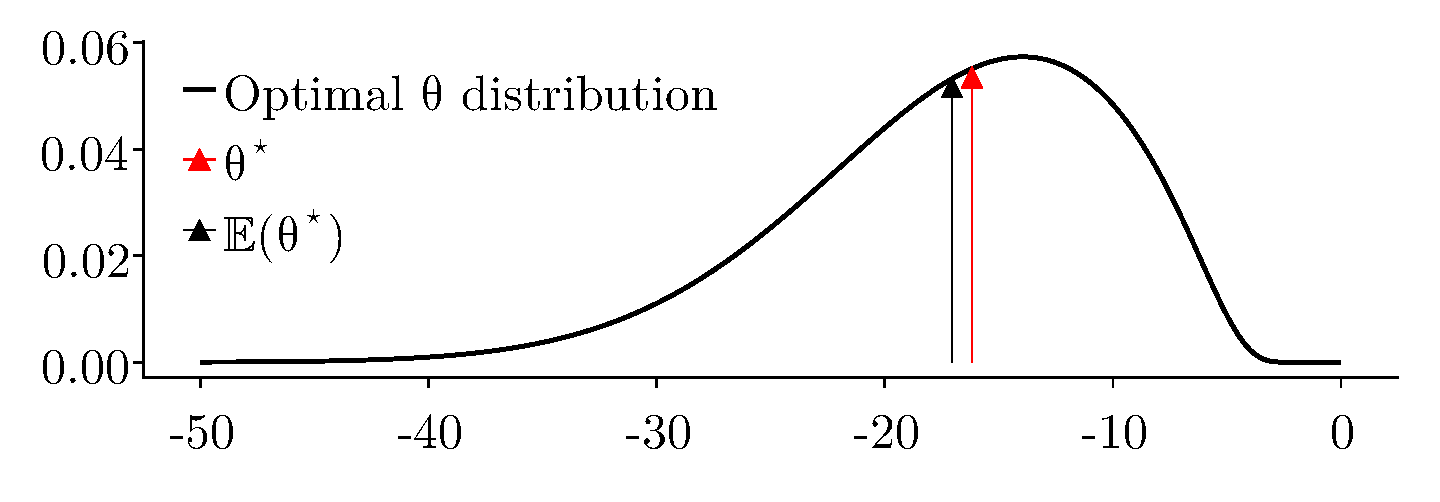
\includegraphics[width=0.7\linewidth]{./figures/optimal-dist.eps}
  \caption{The optimal control parameter distribution given that the system
  parameter $p$ is normally distributed with mean $\hat{p} = 5$ and $\sigma_p
  = 5$. The red and black arrows respectively indicate the optimal control
  parameter without considering the randomness of $p$, and the expected value
  of the optimal control parameter distribution.}
  \label{fig:optimal_dist}
\end{figure}


There are several advantages of employing Bayesian learning to find the optimal
control parameter $\theta$ as the toy example in this subsection supports. 
%
In order to derive some quantitative results, let us assign some numerical
values to the parameters that define the optimal cost function $(q,r) = (100, 1)$, our best
guess $\hat{p} = 5$ of the system parameter $p$ and its standard deviation $\sigma_p = 5$.


The optimal control parameter and cost derived for this system whose model is
assumed to be known perfectly are given by $\hat{\theta}^\star = -16.180$ with
the corresponding estimated cost $\hat{\mc{J}}^\star = 8.090$.
%
This deterministic performance estimate turns out to be \textit{overconfident} when
uncertainties in the system parameter are present. 
%
For example, if the prior knowledge on the distribution of the system parameter
$p$ is utilized, the expected value of the controller parameter is found as
$\mathbb{E}[\theta^\star] = -17.046$ and the corresponding expected cost is
$\mathbb{E}[\mc{J}] = 8.523$. 
%
The controller from the deterministic training/optimization is not only
overconfident about its performance; but also is less robust against modeling
errors, as the Bayesian learning yields a closed-loop stable system for a wider
range of values of $p$.

Finally, Figure~\ref{fig:optimal_dist} shows the optimal control parameter
distribution given that the system parameter $p$ is normally distributed with
mean $\hat{p} = 5$, standard deviation $\sigma_p = 5$.
%
This figure also shows the mean values of the optimal control distribution with
the black arrow and the optimal control parameter a deterministic approach would
yield in red. 
%
We notice that the Bayesian learning that yields the optimal control parameter
distribution is more concerned about system stability due to the uncertainty in
the parameter $p$, a feat that the deterministic training may not reason about.

\subsection{Optimal Control under Parameter Uncertainty and Measurement
Noise}

Consider the scenario in which the system~\eqref{eq:first-order} is also subject
to measurement errors; that is, our measurement model for the state $x$ is
probabilistic and is distributed according to the Gaussian $\mc{N}(x,
\sigma^2)$. Since the controller uses this measurement to determine its action,
the closed-loop system has to be modelled as a stochastic differential equation
(SDE), given by
%
\begin{equation} \begin{cases} dx(t) =
(p+\theta)x(t) \; dt + \theta\sigma \; dW_t, \\ x(0) = 1,
\end{cases} \label{eq:first-order-SDE} \end{equation}
%
where $W$ denotes the Wiener process~\cite{evans2012introduction}. The initial
state is assumed deterministic and is set to unity for simplicity.  
% The general case where the initial state is arbitrary and
% stochastic follows exactly the same lines of development.
% 
The unique solution to this SDE is given by
%
\begin{equation}
    x(t) = e^{(p+\theta)t} + \theta\sigma \int_0^t e^{(p+\theta)(t-s)}dW_s.
    \label{eq:sol-sde}
\end{equation}
%
\vspace{-4mm}
\begin{lem}\label{lem:1}
    The conditional expectation $\mathbb{E}\left[\mc{J}\mid p\right]$ of the
    performance index~\eqref{eq:perfind} given the system parameter $p$ is 
    \begin{align*} 
      \mathbb{E}\left[\mc{J} \mid p\right] &=-\frac{1}{4}\frac{q+r\theta^2}{p+\theta}
       \left[ \theta^2 \sigma^2 T + \left(1 - e^{2T(p+\theta)}\right) \left(1 +
      \frac{1}{2}\frac{\theta^2\sigma^2}{p+\theta}\right)\right].  
    \end{align*} 
\end{lem}
%

\begin{proof}
    The proof may be found in the appendix.
\end{proof}
%

%
It is easily shown that this quantity is positive for all $T>0$. Furthermore, it
blows up as the horizon $T$ is extended to infinity. This is not surprising
since a nonzero measurement noise causes the state to oscillate around the
origin, rather than asymptotically converging to it, incurring nonzero cost
all the while.

% As a concrete example, take the values of $q$, $r$ and $p=\hat{p}$ as in
% Table~\ref{tab:case-study} and further let $T=1$ and $\sigma = 0.2$. In this
% case, the deterministic optimal for the controller parameter is
% $\theta_d^\star = -10.916$. Selecting this controller parameter incurs an
% expected cost $\mathbb{E}_W\left[\mc{J}(\theta_d^\star) \mid p \right] =
% 31.473$. On the other hand, the actual (stochastic) optimal of the controller
% parameter may be found by minimizing $\mathbb{E}_W\left[\mc{J} \mid p \right]$
% numerically and it yields $\theta_s^\star = -7.331$ with an expected cost
% $\mathbb{E}_W\left[\mc{J}(\theta_s^\star) \mid p \right] = 21.399$, which is
% smaller than the one provided by the deterministic optimal. 

We have kept the system parameter $p$ constant in this analysis so far.
Uncertainty over this variable can be incorporated by taking a further
expectation \[ \mathbb{E}[\mc{J}] := \mathbb{E}_p\left[\mathbb{E}_W\left[\mc{J}
\mid p \right]\right], \] of $\mathbb{E}_W\left[\mc{J} \mid p \right]$ over $p$,
which must be accomplished numerically as it does not admit a closed-form
expression.  

We can then minimize $\mathbb{E}[\mc{J}]$ over the control parameter in order to
study the effects of both kinds of uncertainties on the optimal controller.
%
Such a study is provided in Figures~\ref{fig:iwp-projections}
and~\ref{fig:iwp-loss}, where we have plotted the optimal control parameter
$\theta^\star$ and the minimal expected cost $\mathbb{E}[\mc{J}]$ as a function
of the standard deviations of the measurement noise $\sigma$ and the system
parameter $\sigma_p$. The constants we used to generate the data are given by
$q=r=1$ and $T=\hat{p}=3$. Our first observation is that the magnitude of the
optimal control parameter is an increasing function of system parameter
uncertainty and a decreasing function of measurement uncertainty. Our second
observation is that if the measurement noise is small, then the optimal control
parameter is insensitive to system parameter uncertainty as long as this
uncertainty is small. The optimal cost shares this insensitivity for an even
wider range of values of $\sigma_p$. In a similar vein, if the uncertainty in
the system parameter is large, then the optimal control parameter is insensitive
to the magnitude of the measurement noise. However, the optimal cost is still
sensitive to this quantity.

\begin{figure}[tb]
  \centering
    \begin{minipage}{.48\textwidth}
        \centering
        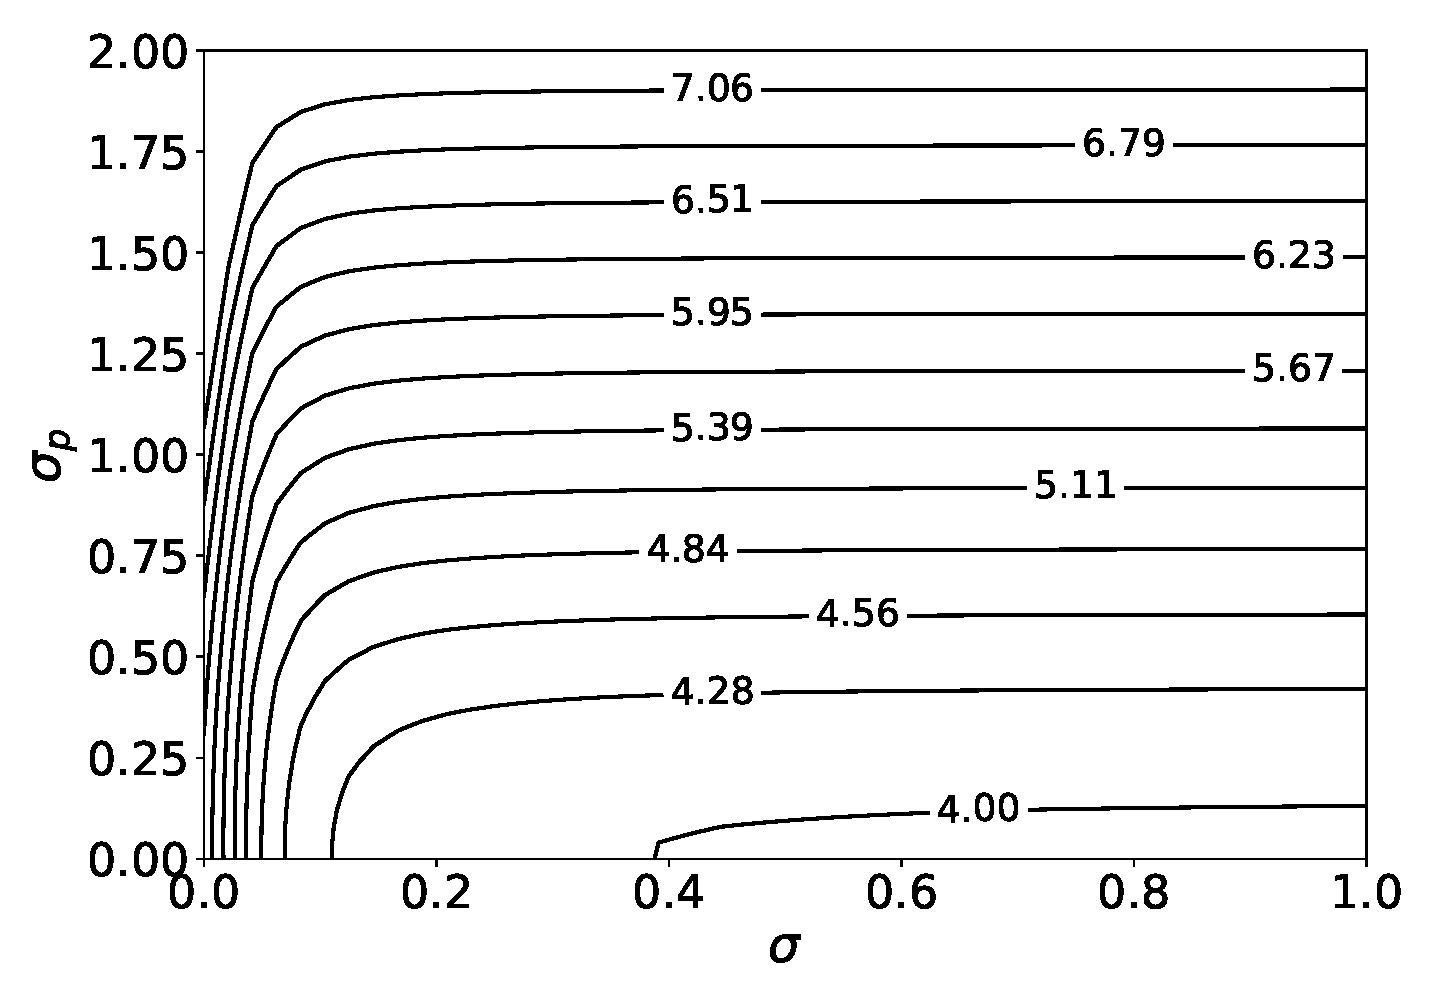
\includegraphics[width=\linewidth]{./figures/optimal_ctrl.eps}
        \caption{The optimal controller parameter magnitude $\abs{\theta^\star}$.}
        \label{fig:iwp-projections}
    \end{minipage}%
    \hfill
    \begin{minipage}{0.46\textwidth}
        \centering
        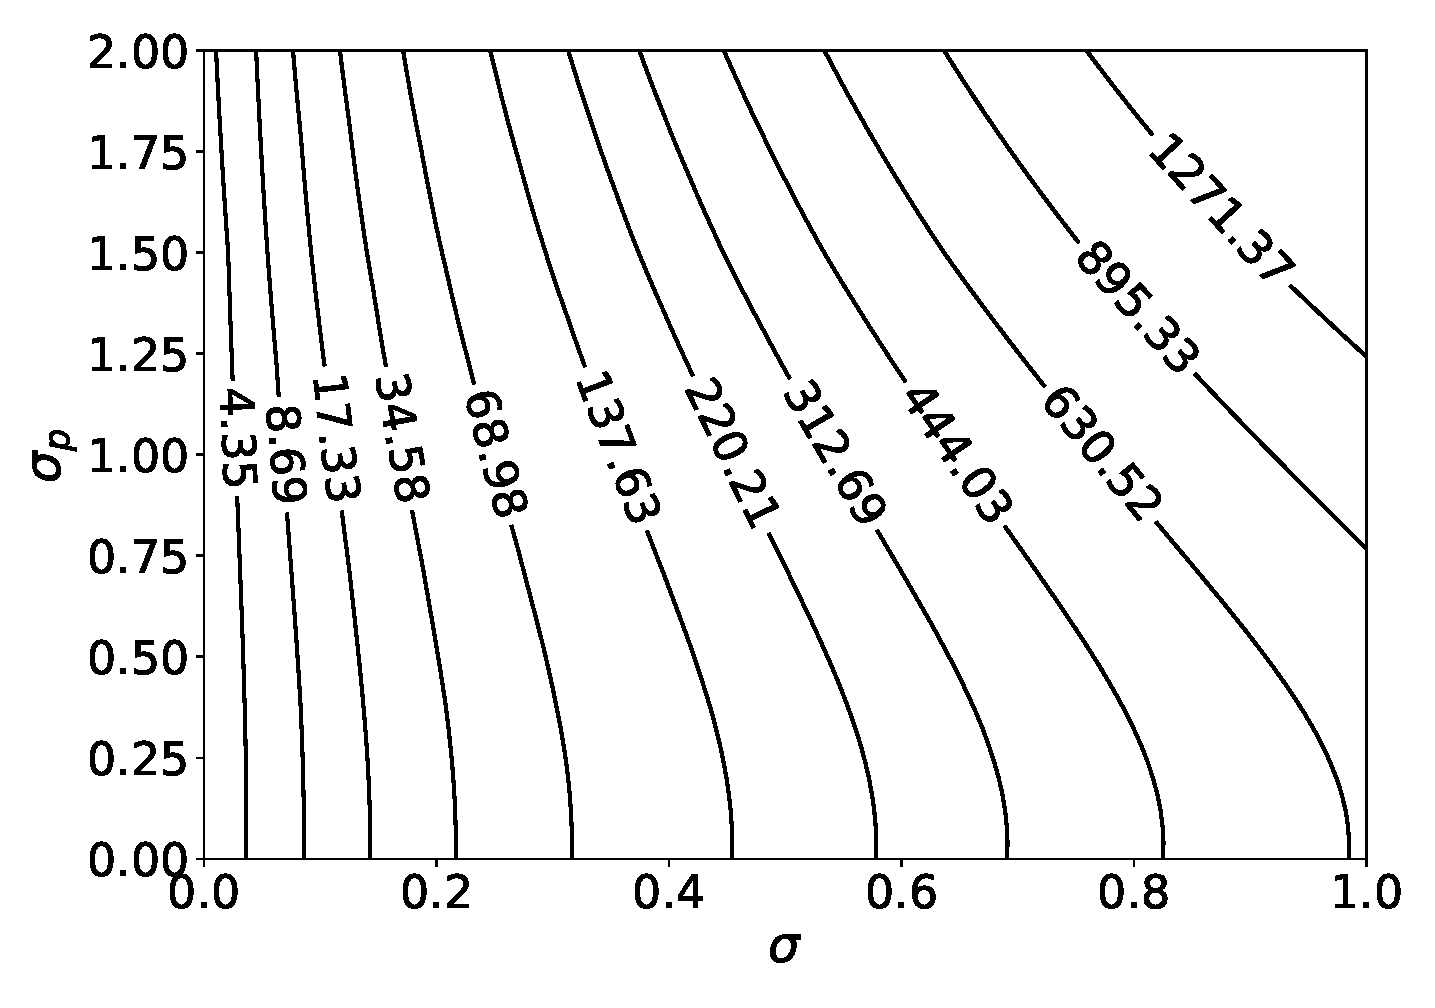
\includegraphics[width=\linewidth]{./figures/optimal_cost.eps}
        \caption{The minimal expected cost $\mathbb{E}[\mc{J}]$.}
        \label{fig:iwp-loss}
    \end{minipage}
  % \caption{As a function of the standard deviations of the measurement noise,
  %   $\sigma$, and the system parameter, $\sigma_p$ (a) the magnitude of the optimal
  %   controller parameter $\abs{\theta^\star}$ and (b) the minimal expected cost 
  %   $\mathbb{E}\mc{J}$.}
  %
  \label{fig:optimal-ctrl-cost}
\end{figure}

% \begin{figure}[]
%     \centering
%     %
%     \setkeys{Gin}{width=0.48\linewidth}
%     \subfloat[The optimal controller parameter magnitude $\abs{\theta^\star}$.]
%     {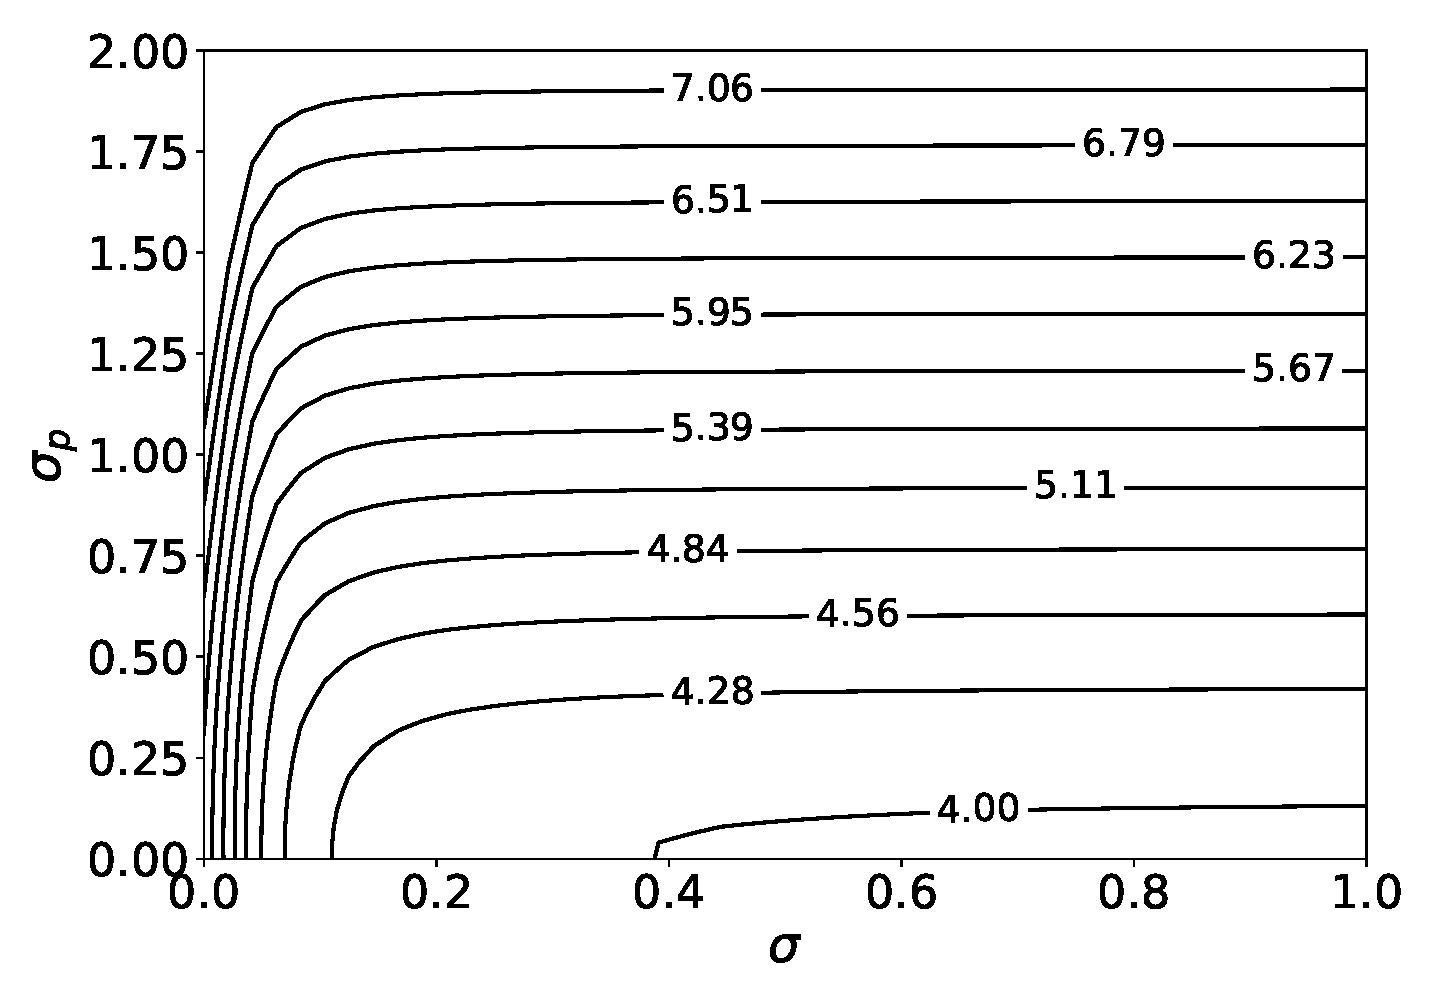
\includegraphics{./figures/optimal_ctrl.eps}}
%     % \label{fig:iwp-projections}
%     %
%     % \hspace{5pt}
%     \hfill
%     %
%     \subfloat[The minimal expected cost $\mathbb{E}\mc{J}$.]
%     {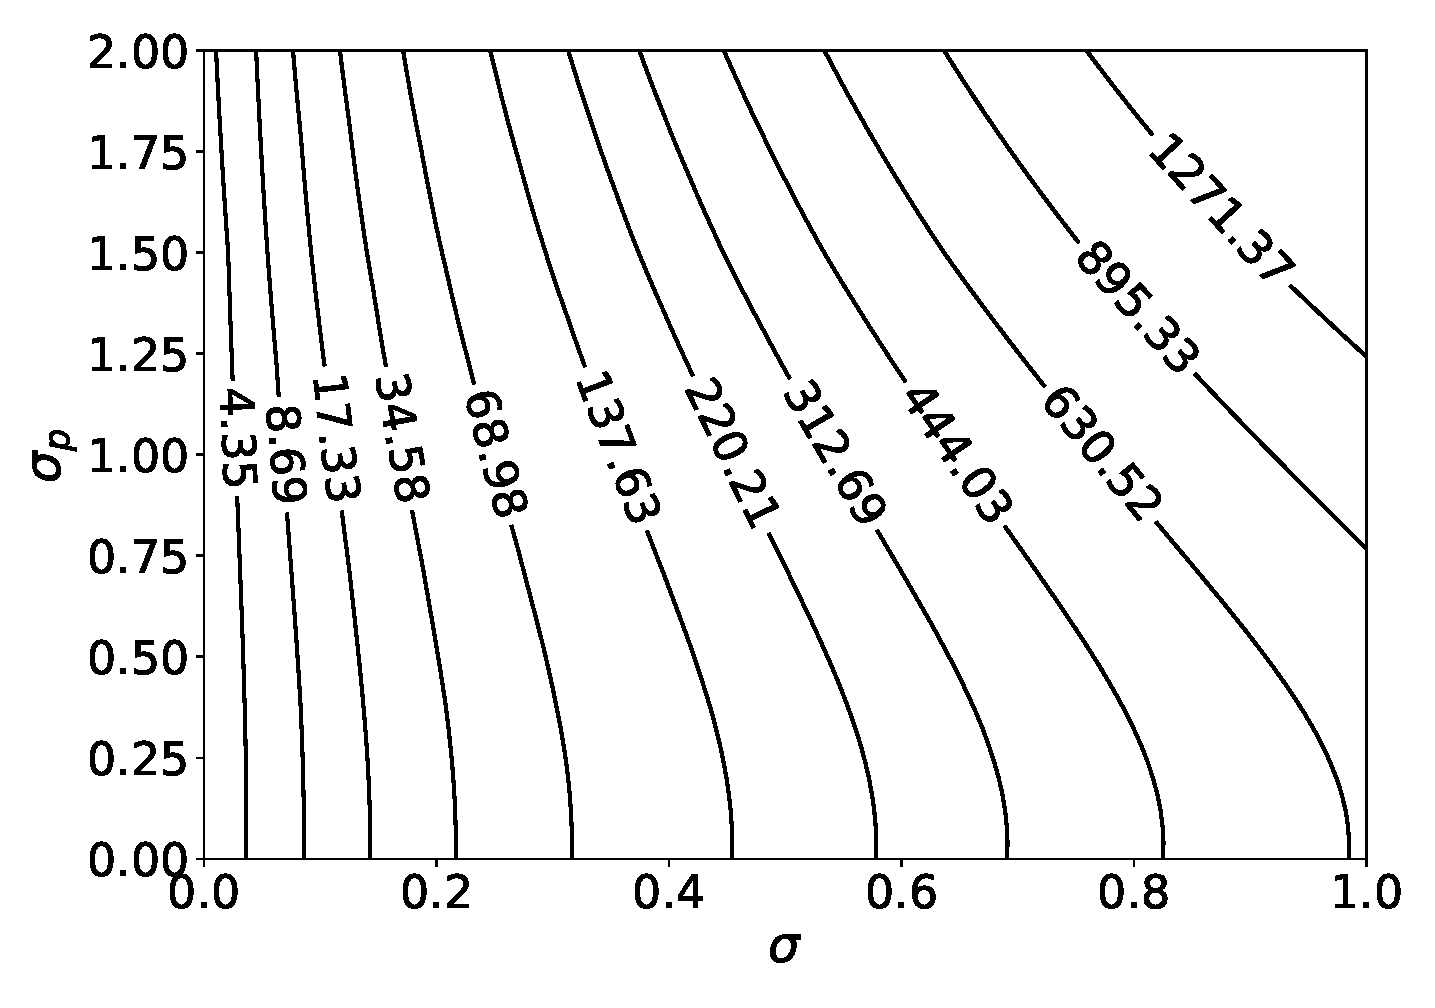
\includegraphics{./figures/optimal_cost.eps}}
%     % \label{fig:iwp-loss}
%     %
%     \caption{As a function of the standard deviations of the measurement noise,
%     $\sigma$, and the system parameter, $\sigma_p$ (a) the magnitude of the optimal
%     controller parameter $\abs{\theta^\star}$ and (b) the minimal expected cost 
%     $\mathbb{E}\mc{J}$.}
%     %
%     \label{fig:optimal-ctrl-cost}
% \end{figure}

\section{Neural Bayesian Learning}

In Section~\ref{sec:justification}, we have shown that optimal deterministic
policies are less robust against system parameter uncertainties and measurement
noise than Bayesian policies. Hence, we introduce a Bayesian framework that
combines the power of data-driven deterministic techniques with Bayesian
learning. In this technique, we inject model and measurement uncertainties
directly into the training loop in order to learn a stochastic controller that
works for a wide range of system parameters and measurement noise. We refer to
this Bayesian technique as Neural Bayesian Learning (NBL). NBL poses the control
search problem as the following optimization problem.

\begin{equation}
    \begin{aligned}
        \underset{q(\theta) }{\textrm{minimize}} 
        &&\quad J(&\phi(t; x_0, u), u) \\
        \textrm{subject to} 
        &&\quad \dd {x} &= f(x, u; \zeta) \dd t + \nabla_x u(x) \dd W_t, \\
        &&\quad u(x; \theta) &= g \circ F(x; \theta), \\
        &&\quad \zeta &\sim \mathcal{N}(\zeta_0, \sigma_\zeta), \\
        &&\quad \theta &\sim q(\theta),
    \end{aligned}    
    \label{eq:neural_bayesian_inference}%
  \end{equation}
%
where $J(\phi(t; x_0, u), u)$ is the running cost function given the flow of the
system $\phi(t; x_0, u)$ under the control input $u$, $f$ is the dynamics of the
robot with system parameters $\zeta$ sampled from normal distribution
$\mathcal{N}$ with nominal system parameters $\zeta_0$ and system parameter
uncertainty $\sigma_\zeta$. The target function $F$ is a BNN whose parameters
are samples drawn from the posterior distribution $q(\theta)$ and $g$ is the
mapping from the learned target function $F$ to the control input. The equations
of motion of the robot are given by stochastic differential equations (SDE)
that model measurement error by the Wiener process $\dd W_t$; $\nabla_x u(x)$ is
the coefficient of the first-order Taylor approximation of $u(x)$ around zero
noise. The NBL technique adapts additional constraints from other deterministic
control design techniques, such as \textsc{NeuralPbc} and \textsc{Neural-IdaPbc}.
The objective is to learn the probability distribution over the parameters of
$F$ for a wide range of system parameters $\zeta$ and measurement error. For
most dynamical systems, a closed-form solution to the optimization problem
in~\eqref{eq:neural_bayesian_inference} is intractable. Hence, we devise the
procedure outlined in Algorithm~\ref{algo:nbl} to obtain the solution to the
optimization problem. 

As shown in Algorithm~\ref{algo:nbl}, we begin the NBL procedure with a choice
of a prior distribution. We take two approaches to selecting the prior
distribution $p(\theta)$. The simplest approach is to use an uninformed prior
with randomly initialized distribution parameters to start the optimization
problem; this choice encourages exploration but has slow convergence properties.
The second approach uses an informed prior that warm-starts the Bayesian
training around the solution of a deterministic training. To do so, the prior
distribution parameters are selected such that it is centered around the
parameters learned from a deterministic technique such as \textsc{NeuralPbc} or
\textsc{Neural-IdaPbc}.

In order to collect training data, we sample the state space for initial states
$x_0$ and save them in the dataset $\mathcal{D}$. There are few options to
efficiently sample the state space, three of which are discussed in the
following section.

\subsection{Sampling initial states}
\label{ssec:state_sampling}

The loss function in~\eqref{eq:xperploss} depends on the initial state
through the prediction $\gamma : t \to \phi(t; x_0, u^\theta)$. 
%
Let $N_\mathcal{D}$ denote the size of the training data $\mathcal{D}$. 
%
Instead of randomly sampling the entire space for initial state $x_0$, we adopt
one or a combination of the state sampling techniques from~\cite{neuralpbc},
\cite{datadriven_ESC} and \cite{DBLP:journals/corr/abs-1011-0686}. Three of
these techniques are discussed as follows.
%
\begin{enumerate}
    \item \textsc{DAgger}~\cite{DBLP:journals/corr/abs-1011-0686}: this strategy
    samples a collection of initial states $\{x_0\}$ from trajectories
    $\{\gamma\}$ generated by executing the current policy $u^\theta$. This
    iteratively collects new samples from the regions of the state-space visited
    by the learned controller. 
    \item Sampling around desired equilibrium~\cite{neuralpbc}: this technique samples from $x_0
    \sim \mathcal{N} \left(x^\star, \Sigma_0\right)$, where the variance $\Sigma_0$
    is kept small. Sampling initial states from $x_0 \sim \mathcal{N}
    \left(x^\star, \Sigma_0\right)$ helps recover from locally optimal solutions
    obtained from trajectories that predominantly miss the goal set
    $\mathcal{S}$ by a large amount. As the learning proceeds, we gradually
    switch to the \textsc{DAgger} sampling strategy. 
    \item Sampling from expert trajectory~\cite{datadriven_ESC}:  
    Similar to sampling around desired equilibrium, this technique helps recover
    from locally optimial solutions. Early in the learning process, we uniformly
    sample the state space and produce expert trajectories from the path
    planner. The points along these trajectories are then used as
    \textit{initial states} for generating $\gamma$ to be included in the
    computation of the loss. This kick-starts the learning process with several
    samples already close to the goal set. As the learning proceeds, we
    gradually switch to the \textsc{DAgger} sampling strategy. 
\end{enumerate}

After each iteration through the entire dataset, we substitute $N_{\textrm{R}}$
points in $\mathcal{D}$ with new samples, keeping an $N_\mathcal{D} -
N_\textrm{R}$ portion of initial states as the \textit{replay buffer}, a common
technique used in reinforcement learning algorithms~\cite{lin1992self}.

Once we collect initial states in $\mathcal{D}$, we randomly select $d$ batches
from the dataset and generate trajectories using the current policy parameter
$\theta$ sampled from the posterior $p(\theta | \mathcal{D})$. For each initial
state in $d$, a new system parameter $\zeta$ is sampled from the distribution
$\mathcal{N}(\zeta_0, \sigma_\zeta)$. The running cost $\mathcal{J}$ is the sum
of the cost of each trajectory created from the batch $d$. There are various
ways to design the cost function $J$, three of which are discussed as follows.

\subsection{Cost Function}
\label{ssec:cost}

The cost function $J$ helps impose various desired behaviors in the learned
controller. In this section, we present three performance objectives, their
corresponding likelihood functions and the desired behavior they impose.

\begin{enumerate}
    \item Trajectory tracking: Let $x^\star$ denote the desired equilibrium of a
    dynamical system and $\gamma : t \to \phi(t; x_0, u^\theta)$ represent a
    prediction from the initial condition $x_0$ with the current control law
    $u^\theta$. The objective of this task is to find a closed-loop controller
    that can track an expert trajectory $\gamma^\star$ obtained from a path
    planner. To impose this behavior, the running cost is a function of the
    distance from the current trajectory $\gamma$ to $\gamma^\star$, defined in
    terms of the transverse coordinates $\gamma_\bot-\gamma^\star_\bot$ along
    the preferred orbit, using the ideas outlined
    in~\cite{shiriaev2009transverse,manchester2010transverse}. In this setting,
    the prediction converges to $\gamma^\star$ if and only if
    $\gamma_\bot-\gamma^\star_\bot \xrightarrow{t \to \infty}{} 0$. In order to
    encourage this behavior, we define the cost function as
    %
    \begin{equation}
        % J_{\textrm{MSE}} =  \frac{1}{N} \sum_{n=0}^N \Big( \norm{x(t_n) - \hat{x}(t_n)}{} + \norm{u(t_n) - \hat{u}(t_n)}{} \Big)
        J_{track}(\gamma_\bot) =  \sum_{x_\bot \in \gamma_\bot, \; x^\star_\bot \in \gamma^\star_\bot} |\left| x_\bot-x^\star_\bot | \right |^2
        \label{eq:xperploss}   
    \end{equation}
    %
    Thus, the likelihood can be constructed to minimize the cost $J_{track}$ as follows.
    \begin{align}
        p(\gamma_\bot | \theta) = \prod_{x_\bot \in \gamma_\bot, \; x^\star_\bot \in \gamma^\star_\bot}\mathcal{N}(x^\star_\bot , \Sigma),
        \label{eq:track_likelihood}
    \end{align}
    %
    where $\Sigma$ parameterizes the variance of the likelihood. On top of the
    target function parameters $\theta$, we wish to learn the posterior over the
    variance $\Sigma$ of the likelihood. This allows us to adaptively tune the
    weights on the components of $x_\bot-x^\star_\bot$ on the overall cost, such
    that we achieve optimum trajectory tracking. This is most advantageous when
    the states of a system have high variance and the weights on
    $x_\bot-x^\star_\bot$ need to be selected in such a way that one state does
    not dominate the cost $J_{track}$.
    %
    Hence, the posterior distribution $p(\theta | \mathcal{D})$ is a multivariate
    probability distribution over random variable $\xi$, where $\xi = [\theta,
    \Sigma]$.
    \item Set distance loss: Let $\mathcal{S}$ represent a small convex
    neighborhood containing $x^\star$. The objective is to find a policy that
    pulls trajectories to the goal set $\mathcal{S}$. The cost function suitable
    for this task is set distance, $J_{\textrm{set}}$, between the current
    prediction $\gamma$ and the goal set $\mathcal{S}$:
    %
    \begin{equation}
        J_{\textrm{set}}(\gamma)
        = \underset{t}{\inf} \, {\{ \norm{a - b}{}: a \in \gamma(t),\, b \in \mathcal{S} \}}.  
        \label{eq:set_distance}
    \end{equation}
    % 
    For instance, the set $\mathcal{S}$ may be chosen as a ball of radius
    $r$ around $x^\star$ in the standard norm topology. 
    %
    Here, $r$ becomes a hyperparameter of the training algorithm. With a
    particular choice of $\mathcal{S}$, if at any point along the prediction
    $\gamma$, a state $x$ is closer than $r$ to $x^\star$, no penalty is
    incurred by $J_{\textrm{set}}$. The corresponding likelihood function is
    given by 
    \begin{align}
        p(J_{\textrm{set}}(\gamma) | \theta) = \mathcal{N}(0, s^2),
        \label{eq:set_likelihood}
    \end{align}
    where $s$ is a hyperparameter that represents the standard deviation of the
    likelihood.
    %
    \item Terminal loss: encourages trajectories to remain as close to the
    desired state as possible at time $T$. Terminal loss, $\ell_T$, is the
    distance between the final state of the prediction $\gamma$ and $x^\star$,
    which is given by
    %
    \begin{equation}
        J_T(\gamma) = \ell_{\textrm{set}}(\gamma) + \ell_T\left(\gamma\right).
        \label{eq:nn_controller_j} 
    \end{equation}
    %
    The corresponding likelihood function is given by 
    \begin{align}
        p(J_T(\gamma) | \theta) = \mathcal{N}(0, s^2),
        \label{eq:terminal_likelihood}
    \end{align}
\end{enumerate}

\begin{algorithm}[tb]
    \centering
    \setstretch{1.5}
    \caption{Neural Bayesian Learning}\label{algo:nbl}
    \begin{algorithmic}[1]
      \algrenewcommand\algorithmicindent{0em} % No indent
      \Procedure{NBL}{$f,\theta$}
      \State Select prior distribution $p(\theta)$
      \State $f \,\gets f(x, u; \zeta)$ dynamics given by SDE using current policy
      \State $\mathcal{D} \gets \{x_0\}_{(N_{\mathcal{D}})}$  \Comment{$N_{\mathcal{D}}$ samples of $x_0$}
      \algrenewcommand\algorithmicindent{1.5em} % Change indent back to default
      \For{$i=1:\texttt{maxiters}$}
          \For{each $d$ $\subset \mathcal {D}$} \Comment Select batch $d$ from dataset $\mathcal{D}$
              \State Initialize $\mathcal{J} = 0$
              \State $\theta \sim p(\theta | \mathcal{D})$ \Comment{Sample parameters of $F$ from posterior}
              \For{each $x_0 \in d$}
      % \algrenewcommand\algorithmicindent{1.5em} % Change indent back to default
                  \State $\zeta \sim \mathcal{N}(\zeta_0,\sigma_{\zeta})$ \Comment{Sample system parameters}
                  \State $\phi(t; x_0, u) \gets$ integrate dynamics from $x_0$ 
                  \State $\mathcal{J} \gets \mathcal{J} + J(\phi(t; x_0, u), u)$
              \EndFor
          \State Compose likelihood $p(d | \theta)$
          \State Compute joint probability $p(\theta,d) = p(d | \theta) p(\theta)$
          \State Update posterior $p(\theta|\mathcal{D})$ through MCMC or variational inference
          \EndFor
        \State $\mathcal{D} \gets \{\mathcal{D}\}_{(1,\ldots,N_{\mathcal{D}}-N_{\textrm{R}})} \cup \{x_0\}_{(N_{\textrm{R}})}$\Comment{Replay buffer}
      \EndFor
      \State \textbf{return} $q(\theta) = p(\theta|\mathcal{D})$
      \EndProcedure
    \end{algorithmic}
\end{algorithm}

On top of the robustness properties of NBL, we can give stability guarantees of
the inferred controller transparently. To do so, we explore the capabilities of
NBL on frameworks that combine data-driven techniques with passivity-based
control. In the following section, we introduce passivity-based control and the
improvements incorporated from the NBL technique.


\section{Neural Passivity-Based Control (\textsc{NeuralPBC})}
\label{sec:ml-pbc-bayes}
%#########################################################
Let $x \in \mathcal{X} \subset \mathbb{R}^{2n}$ denote the state of the robot.
%
The state $x$ is represented in terms of the generalized positions and momenta
$x = (q, p)$. 
%
With $M$ denoting the symmetric, positive-definite mass matrix, the Hamiltonian
$H$ of the robot is expressed as 
%
\begin{equation}
    H(q,p) = \frac{1}{2} p^\top M^{-1}(q) p + V(q),
    \label{eq:system_hamiltonian}
\end{equation}
%
where $V(q)$ represents the potential energy. The system's equations of motion
can then be expressed as 

%
\begin{align}
    \begin{split}  
      \bmat{\dot{q} \\ \dot{p}} &= \bmat{0 & I_n \\ -I_n & 0}\bmat{\nabla_qH \\
      \nabla_pH} + \bmat{0 \\ G(q)}u, \\
      y &= G^\top \dot{q},
    \end{split}
    \label{eq:hamiltonian_dynamics}
\end{align}
%
where $G(q) \in \mathbb{R}^{n \times m}$ is the input matrix, $I_n$ denotes the
$n \times n$ identity matrix, and $u \in \mathbb{R}^m$ is
the control input.
%
The system~\eqref{eq:hamiltonian_dynamics} is \textit{underactuated} if rank $G
= m < n$.

The main idea of passivity-based control (PBC)~\cite{van2000l2} is to design the
input $u$ with the objective of imposing a desired storage function $H_d:
\mathcal{X} \rightarrow \mathbb{R}$ on the closed-loop system, rendering it
passive and consequently stable.
%
In the standard formulation of PBC, the control comprises an
energy shaping term and a damping injection term:
%
\begin{equation}
  u = u_{es}(x) + u_{di}(x).
  \label{eq:ida-pbc_control}
\end{equation}
%
% such that the closed loop dynamics satisfies
% %
% \[
%   H_d(x(t)) - H_d(x(0)) = \int_0^t u_{di}^\top(t) y(t) \, \dd t - d^\star(x(t)),
% \]
% %
% where $d^\star \geq 0$ is the desired damping dissipation. 
%
For mechanical systems, one solution to the PBC problem is of the form
%
\begin{align*}
  u_{es}(x) &= 
  % -\left( G^\top G  \right)^{-1} G^\top
  -G^{\dagger}
  \left( \nabla_q H_d - \nabla_q H \right), \\
  u_{di}(x) &= - K_{v} \, y,%\quad \mathbb{R}^{m \times m} \ni K_v \succ 0,
\end{align*}
%
where $G^\dagger = \left( G^\top G  \right)^{-1} G^\top$, and $K_v \succ 0$ is the
damping gain matrix. The choice for $H_d$ must satisfy
%
\begin{align}
  G^\bot \left( \nabla_q H_d - \nabla_q H \right) = 0,
  \label{eq:pdes}
\end{align} 
%
where $G^\perp G = 0$, and $H_d$ has a minimum at the desired equilibrium
$x^\star$. However, the closed-form solution to the partial differential
equations (PDEs) in~\eqref{eq:pdes} is intractable. The deterministic
\textsc{NeuralPbc} framework presented in~\cite{neuralpbc} solves the PDEs given
in~\eqref{eq:pdes} by rewriting the PBC problem as an optimization problem of
the form 
\begin{equation}
  \begin{aligned}
      \underset{\theta}{\textrm{minimize}} 
      & & &\int_{0}^{T} \ell \left(\phi,u^{\theta}(\phi) \right) \, \dd t , \\%
      \textrm{subject to}
      & & \dot{x} &= \bmat{\phantom{-}\nabla_p H \\ -\nabla_q H} + \bmat{0 \\ G(q)}u^{\theta}, \\%
      & & u^{\theta} &= -G^{\dagger} \nabla_q H_d^{\theta} - K_v^{\theta} G^\top \nabla_p H_d^{\theta},%
      % & \quad x(0) &= x_0 \in \mathcal{X}, \\%
  \end{aligned}
  \label{eq:neural_pbc_finite_optim}
\end{equation}
where $T>0$ is the time horizon, $\ell: \mathcal{X} \times \mathcal{U}
\rightarrow \mathbb{R}$ is a running cost function to be defined, and $\phi(t;
x_0, u^\theta)$ is the flow of the dynamical system.
%
The \textsc{NeuralPbc} technique adds three important features to the classical 
PBC framework.
\begin{enumerate}
  \item The optimization problem finds an approximate solution to the PDEs in~\eqref{eq:pdes}.
  \item Desired system behavior is explicitly introduced into the optimization via the performance objective $\ell$.
  \item The universal approximation capabilities of neural networks are leveraged to parameterize the desired Hamiltonian $H^\theta_d$.
\end{enumerate}
%############################################################

 
%
With a slight modification to the deterministic \textsc{NeuralPbc} technique, we
can design a controller that is more robust against system parameter
uncertainties and measurement errors via NBL.
%
In the NBL framework outlined in Algorithm~\ref{algo:nbl}, $H^\theta_d$ is the
target function parameterized by a BNN, whose parameters are random variables
sampled from the posterior distribution.
%
The likelihood function that corresponds to the objective function
in~\eqref{eq:neural_pbc_finite_optim} is chosen to be a Gaussian probability
distribution of the form
\begin{equation}
    p(\ell(\gamma, u^\theta) \mid \theta) = \mathcal{N}\left(0, s^2 \right),
    \label{eqn:likelihood_neuralpbc}
\end{equation}
where $\mathcal{N}$ represents the Gaussian probability distribution, and $s$ is
a hyperparameter that represents the standard deviation of the likelihood. The
running cost function $\ell$ is the sum of the set distance loss $J_{set}$ and terminal
loss $J_T$ discussed in Section~\ref{ssec:cost}. While set distance loss
encourages trajectories to approach the neighborhood of $x^\star$ at any point
along the prediction, the terminal loss encourages trajectories to remain as
close to the desired state as possible at time $T$.
%
The running cost $\ell$ is computed for initial states sampled from $x_0 \sim
\mathcal{N}(x^\star, \Sigma_0)$ and \textsc{DAgger} (discussed as methods 2 and
1 in Section~\ref{ssec:state_sampling} respectively).
%##################################################
% \subsubsection{Gradients}
% Similar to the deterministic training, we use the adjoint method to compute the
% gradient ${\partial \mathcal{L}}/{\partial z}$ through the solution of the SDE
% given in~\eqref{eq:sde_initial}.
% %
% Moreover, we invoke the reparameterization trick of the Automatic
% Differentiation Variational
% Inference(\textsc{ADVI})~\cite{kucukelbir2015automatic} to compute the gradient
% of samples $\theta$ with respect to the distribution parameters $z$.

% 
\section{Neural Interconnection and Damping Assignment Passivity Based Control (\textsc{Neural-IDAPBC})}

\textsc{IdaPbc}, a variant of \textsc{Pbc}, selects a particular structure for
$H_d$ 
\begin{equation}
  H_d(q, p) = \frac{1}{2} p^\top M_d^{-1}(q) p + V_d(q),
  \label{eq:idapbc_desired_hamiltonian}
\end{equation}
such that the control input must satisfy the PDEs given by 
\begin{equation}
  G^\perp \left\{ \nabla_qH - M_dM^{-1} \nabla_qH_d + J_2M_d^{-1}p \right\} = 0.
  \label{eq:pde_idapbc}
\end{equation}
The objective is to learn $V_d$ and the entries of $M_d$ and $J_2$ matrices.
Once $V_d$, $M_d$ and $J_2$ are obtained, the energy-shaping control and the
damping injection term are given by
%
\begin{align}
  \begin{split}
  u_{es} &= G^{\dagger} \left(\nabla_qH - M_dM^{-1} \nabla_qH_d + J_2M_d^{-1}p\right), \\
  u_{di} &= -K_v G^\top \nabla_p H_d,
  \end{split}
  \label{eq:idapbc_ues}
\end{align}
%
respectively, where $G^{\dagger} = \left(G^\top G\right)^{-1} G^\top$.

The closed-form solution to the PDEs in~\eqref{eq:pde_idapbc} is intractable.
Hence, the deterministic \textsc{Neural-IdaPbc} framework introduced
in~\cite{neuralidapbc} formulates the following optimization problem that finds
an approximate solution to the PDEs.

\begin{equation}
  \begin{aligned}
      \underset{\theta }{\textrm{minimize}} 
      &&\quad \left\| l_{\textrm{IDA}} (x) \right\|^2 &= \left\| G^\perp \left\{ \nabla_qH - M_dM^{-1} \nabla_qH_d + J_2M_d^{-1}p \right\} \right\|^2, \\
      \textrm{subject to} 
      &&\quad M_d^\theta &= \big( M_d^\theta \big)^\top \succ 0, \\
      &&\quad J_2^\theta &= -\big( J_2^\theta \big)^\top, \\
      % &&\quad q^\star &= \underset{q}{\textrm{argmin}} \; V_d^\theta.  \\
      &&\quad q^\star &= \underset{q}{\textrm{argmin}}\; V_d^\theta.
  \end{aligned}    
  \label{eq:idapbc_finite_optim}%
\end{equation}
where $V^\theta_d$ and the entries of the $M^\theta_d$ and $J^\theta_2$ matrices
are parameterized by neural networks. 

Extending on the \textsc{Neural-IdaPbc} technique, we can find more robust
solutions to the optimization problem via the NBL technique. In the Bayesian
framework outlined in Algorithm~\ref{algo:nbl}, we parameterize the target
function $V_d^\theta$ and the entries of $M_d^\theta$ and $J_2^\theta$ matrices
with BNNs. 
%
The goal is to learn the posterior distribution over the BNN parameters $\theta$
for wide range of system parameters.
%
The likelihood that achieves the performance objective
of~\eqref{eq:idapbc_finite_optim} is chosen to be
%
\begin{equation}
    p(\left\| l_{\textrm{IDA}} \right\|^2 \mid \theta) = \mathcal{N}\left(0, s^2 \right),
    \label{eqn:likelihood_idapbc}
\end{equation}
%
% Unlike the \textsc{NeuralPbc} 